% This is samplepaper.tex, a sample chapter demonstrating the
% LLNCS macro package for Springer Computer Science proceedings;
% Version 2.21 of 2022/01/12
%
\documentclass[runningheads]{llncs}
%
\usepackage[T1]{fontenc}
% T1 fonts will be used to generate the final print and online PDFs,
% so please use T1 fonts in your manuscript whenever possible.
% Other font encodings may result in incorrect characters.
%
\usepackage{graphicx}
% Used for displaying a sample figure. If possible, figure files should
% be included in EPS format.
%
% If you use the hyperref package, please uncomment the following two lines
% to display URLs in blue roman font according to Springer's eBook style:
%\usepackage{color}
%\renewcommand\UrlFont{\color{blue}\rmfamily}
%\urlstyle{rm}
%

\usepackage{algorithm}
\usepackage{algpseudocode}
\usepackage{amsmath}

\begin{document}
%
\title{Estimating the Quality of Translated Texts using Back Translation and Resource Description Framework}
%
%\titlerunning{Abbreviated paper title}
% \titlerunning{GATE Framework For Translation Quality Estimation}
\titlerunning{GATE:~Translation Quality Estimation Using RDF}
% If the paper title is too long for the running head, you can set
% an abbreviated paper title here
%
\author{Vinay Neekhra\inst{} \and
Dipti Misra Sharma\inst{}}


% \author{Vinay Neekhra\inst{1}\orcidID{0000-1111-2222-3333} \and
% Second Author\inst{2,3}\orcidID{1111-2222-3333-4444} \and
% Third Author\inst{3}\orcidID{2222--3333-4444-5555}}
%
\authorrunning{V. Neekhra et al.}
% First names are abbreviated in the running head.
% If there are more than two authors, 'et al.' is used.
%
\institute{
Language Technology Research Center (LTRC)\\ Kohli Center on Intelligent Systems (KCIS)\\
International Institute of Information Technology, Hyderabad, India
\email{vinay.neekhra@research.iiit.ac.in}\\ 
% \url{http://www.springer.com/gp/computer-science/lncs} \and
% ABC Institute, Rupert-University Heidelberg, Heidelberg, Germany\\
% \email{\{abc,lncs\}@uni-heidelberg.de}}
\email{dipti@iiit.ac.in}}
%
\maketitle              % typeset the header of the contribution
%
\begin{abstract}How can we effectively estimate the quality of translated texts in the medical field, where back-translation is usually available and/or recommended for sensitive documents. This paper proposes a novel metric, GATE\footnote{GATE:~Graphical Assessment for Translation quality Estimation}, for translation quality estimation task, leveraging the Resource Description Framework (RDF) to encode both semantic and syntactical information of the original and back-translated sentences into RDF graphs. The distance between these graphs is measured to get the semantic similarity score to assess the quality of the translation. Unlike traditional metrics like BLEU and METEOR, our approach is reference-less, capturing both semantic and syntactical information for a comprehensive assessment of translation quality. Our results correlate better with human judgment, giving a better Pearson correlation (0.357) as compared to BLEU (0.200), thereby showing \textasciitilde70\% improvement over BLEU.\@ Our research shows that, in the field of translation evaluation, existing resources like  back-translation  and RDF could be useful.

\keywords{Resource Description Framework (RDF) \and Back Translation \and Translation Quality Estimation \and GATE
%  \and Translation Evaluation
 }
% First keyword  \and Second keyword \and Another keyword.}
\end{abstract}
%
%
%
% ===

% VINAY
% Introduction:
% 1. What is the problem?
% 2. What is Back Translation
% 3. Why Translation Evaluation is important/Motivation to solve this problem
% 5. What I am proposing? - metric built on RDF
% 6. Structure of the paper
\section{Introduction} 

A drug trial in the medical domain incorporates a mandatory consent form called a Medical Consent Form (MCF), which informs the patient about the experiment and its potential side effects. There is a legal requirement for the MCF to be in the patient’s mother tongue and for it to be easy to understand. A human translator translates the original MCF into the patient's mother tongue. As MCFs are sensitive documents, evaluating the quality of translated texts is crucial to ensure faithfulness to the original texts (see Section~\ref{whyevaluate} for an example). 

One way to evaluate the quality of the translated texts is using back-translation (see Section~\ref{BTintro}), wherein the translated text is translated back into the original language. The original and back-translated texts are then compared to estimate the quality of the translation. Back-translation is a prominent way to assess the quality of translated texts in domains, such as medical documents, where accuracy and precision are paramount~\cite{whyBT}\cite{whyBTMedical}.

Experienced professionals are responsible for carrying out all three procedures (see Figure~\ref{figureBT}), namely: initial translation from the source language to the target language, followed by translation from the target language back to the source language, and ultimately, comparison between the original text and the back-translated texts. Our efforts are focused on reducing the efforts of human evaluators comparing the original and back-translated texts by automating the task of evaluating the quality of translated texts.

In this paper, we propose a novel translation evaluation metric, GATE (Graphical Assessment for Translation quality Estimation), which leverages back-translation (see Section~\ref{BTintro}) and the Resource Description Framework (RDF) (see Section~\ref{rdfintro}). GATE encodes both semantic and syntactical information of the original and back-translated sentences into RDF graphs, allowing for a reference-less, semantically-aware assessment of translation quality.

For sensitive documents in the medical field, such as medical consent forms and qualitative research, back-translation is a common practice to ensure the faithfulness of translations~\cite{whyBT}\cite{whyBTMedical}. GATE capitalizes on this by integrating back-translation into its evaluation framework, providing a comprehensive and reliable assessment of translation quality. To estimate the quality of translated texts, we encode the meaning of these sentences into graphs using the Resource Description Framework (RDF) and then compare these graphs to come up with a similarity score (See Figure~\ref{graphcompare}). GATE shows a higher correlation (0.357) with human judgment than BLEU (0.200).\@ (see Section~\ref{experiments} for the experiment details). In the next Section~\ref{whyevaluate}, we discuss the significance of translation evaluation, highlighting the context and motivation behind our research efforts. 


\subsection{Significance of Translation Evaluation}\label{whyevaluate}
% \textcolor{teal}{!Guide is saying that this section is not required, as importance of translation is implicit}\\
Consider the following sentence from a medical consent form for a vaccine trial, translated to the patient’s mother tongue \textit{(Tamil language)} where the original consent form is in English.\\

• \textit{Source text: }\\\quad \textbf{There are no side effects mentioned previously.}\\

To comply with legal requirements, the consent form was translated into Tamil by hospital authorities, resulting in two translated versions. For evaluating the translation quality, the translated MCF was back-translated to English, yielding the following results:\\

\pagebreak
• \textit{Back Translation 1: }
\newline\quad\textbf{No side effects which were mentioned previously}
\\\\
• \textit{Back Translation 2: }
\newline\quad\textbf{It has been already mentioned that it does not have any side-effects}
\\

As seen above, the first back-translated sentence is semantically similar to the source text and preserves the original intent. The second back translated text, on the other hand, conveys that \textit{---as previously mentioned, there are no side-effects---}, whereas the original intent was that no side-effects have been observed yet, thus raising ethical and legal concerns. 

\paragraph{} Thus, it is crucial, that translated texts are evaluated for their faithfulness to the original text, especially in the medical domain. In the next subsection, we highlight the contributions of our work. 

\subsection{Contributions}\label{contri}

\begin{enumerate}
  \item This paper presents a novel approach, GATE, for translation quality estimation task by utilizing back-translation and leveraging knowledge graphs (namely, Resource Description Framework) for encoding the meaning of original and back-translated texts to come up with a translation quality estimation score.
  \item GATE incorporates both syntactic and semantic information, leading to improved evaluation scores. Our approach is applicable to both machine-translated and human-translated texts. Our experiments demonstrate a better correlation with human judgment compared to BLEU, with a Pearson correlation of 0.357 compared to the most commonly used metric, BLEU’s 0.200.
  \item Our approach eliminates the need for reference texts by comparing the source text directly with its back-translated counterpart. This makes our approach reference-less and thus valuable for scenarios where reference texts are not available for translation evaluation (such as medical consent forms).   
  \item While our results do not surpass the current state-of-the-art, our metric, GATE, offers distinct advantages such as requiring no training, being computationally lightweight, being available for low-resource languages, and operating without the need for extensive training data, unlike neural network-based methods like COMET~\cite{comet}.
\end{enumerate}

The paper is structured as follows: Section~\ref{relatedwork} reviews related work in the area of translation evaluation, discussing the limitations of existing metrics. Section~\ref{prelim} builds the foundation of our work, providing an overview of back-translation along with its significance, introduces Knowledge Graphs in general, and describes Resource Description Framework (RDF) and FRED RDF graphs. Section~\ref{experiments} details the experiment design and methodology leading to the creation of GATE.\@ The results of our experiments are presented in Section~\ref{results}, along with a discussion of the insights gained from our research efforts while also addressing the current limitations of our metric. Finally, Section~\ref{conclusion} and Section~\ref{future} conclude the paper along with outlining the directions for future research. 

% \paragraph{}

% \textbf{Once the translation is done, an evaluation is required to assess the quality of translated texts with respect to original text. Human evaluation has been the de-facto standard for translated texts since the need for translation arose. Human evaluation is often expensive, time consuming, subjective, and prone to individual variations (REF??) To address these concerns, a metric is required to evaluate the quality of translation to measure semantic equivalence, with high correlation with human judgment. Many automatic translation evaluation metrics have come up such as BLEU(REF??), METEOR(REF??). However, many of them either require reference text for comparison and/or they don’t consider semantic information for the evaluation??  Once the translation is done, translation evaluation is done using automatic metric like BLEU [1], METEOR [2] in addition to human evaluation. These existing automatic methods often focus on surface-level similarity or require reference translations, limiting their ability to capture the nuances of meaning essential in medical and legal documents.
% Our work mainly focuses on formal documents (such as legal and medical documents), as for these texts, back-translation is usually available and/or recommended.  This paper proposes a novel translation evaluation metric that leverages Resource Description Framework (RDF) and back-translation to provide a reference-less, semantically aware assessment of translation quality.
% However for sensitive documents, human evaluation is de-facto standards. Usually for the texts in medical and legal documents such as qualitative research, medical consent forms, back translation is also usually provided to thoroughly verify the faithfulness of translated text with respect to the original translation [3][4]
% }


% Human evaluation to check the quality of translation is extensive but expensive. Once the translation is done, an evaluation is required to assess the faithfulness of translated texts with respect to original text. Thus, translation evaluation is an important aspect and the human evaluation has been the de-facto standard for translated texts since the need for translation arose. Human evaluation is often expensive, time consuming, and often unreliable ?? To address these concerns, many automatic translation evaluation metrics have come up. However, many of them either require reference text for comparison and/or they don’t consider semantic information for the evaluation?? 

% a metric is required to evaluate the quality of translation to measure semantic equivalence, with high correlation with Human judgment. Our work mainly focuses on formal documents (such as legal and medical documents) as they are generally less ambiguous and legally important. For these texts, back-translation is usually available. 

% Once the translation is done, translation evaluation is done using automatic metric like BLEU \cite{bleu}, METEOR \cite{meteor} in addition to human evaluation. However for sensitive documents, human evaluation is de-facto standards. 


% \paragraph{}
% The structure of the paper is as follows. In next subsections we explain the back translation the Significance and rationale behind it, in section 2, we review related work done in the field of translation evaluation as a broad field. In Section 3, we describe our method and motivation behind it. In Section 4, we explain our experiment design and preprocessing. In Section 5, we present the results of our experiments. In the last Section, we conclude our paper, followed by future work and references. 


\section{Related work}\label{relatedwork}

Existing metrics for translation evaluation, such as BLEU\cite{bleu}, METEOR\cite{meteor}, NIST\cite{nist}, and TER\cite{TER}, have been widely utilized in the field, with BLEU being the most commonly used among them. BLEU compares the translated sentence with a reference sentence. It operates on word group matching using an n-gram model and remains popular due to its simplicity. In contrast, METEOR was developed as a successor to BLEU to account for synonyms and other variations in language. Usually, the quality of translation is evaluated at the sentence level, but word and document level QE are also possible~\cite{specia18}.

However, these metrics have inherent limitations. Many traditional metrics are categorized as n-gram matching metrics, relying on handcrafted features to estimate translation quality by counting the number and fraction of n-grams shared between a candidate translation hypothesis and one or more human references. This restricts their ability to capture nuanced meaning, particularly in complex and domain-specific texts. They often rely on surface-level similarity measures and may necessitate reference translations, typically provided by humans as a standard of perfection. 

More recent approaches have explored the use of word embeddings as an alternative to n-gram matching for capturing word semantic similarity. Metrics like BLEU2VEC\cite{bleu2vec}, BERT SCORE\cite{bertscore}, and COMET\cite{comet} create alignments between reference and hypothesis segments in an embedding space to compute a score reflecting semantic similarity. COMET, a notable metric in this domain, has demonstrated remarkable results for translation evaluation. However, to train these models, the availability of word embeddings for low-resource languages remains a significant challenge. 

However, these metrics may still need to catch up in capturing the full range of nuances captured by human judgments. 
Challenges with existing metrics include their reliance on reference texts for comparison, requiring semantic exactness at the word level, susceptibility to differences in lexical structure (such as word order), and the tendency to measure semantic relatedness rather than semantic similarity, huge data requirement for training models thus not well-suited for low-resource languages.

% VINAY- below line would confuse. It's better not to add. 
% Translation Evaluation on the other hand compares the translated text with the reference text for evaluating the translation quality.

% Leveraging multilingual pretrained encoders, such as multilingual BERT, has shown promising correlations with human judgments in recent studies.

% There are various existing metrics such as: BLEU, NIST, METEOR, TER etc. BLEU being the most popular and most used.


% Existing automatic metrics like BLEU\cite{bleu} and METEOR\cite{meteor} have been widely used for translation evaluation, but they have limitations. These metrics often rely on surface-level similarity measures and may require reference translations, making them less effective in capturing the nuances of meaning, especially in complex and domain-specific texts.

% BLEU was one of the first metrics introduced for translation evaluation task. BLEU compares the translated text with a reference translation (often given by humans as a perfect translation). BLEU is based upon word group matching (n-gram model). BLEU remains one of the most popular and widely used metric for translation evaluation due to its simplicity. 

% METEOR metric was introduced as a successor to BLEU to consider synonyms etc. 
% Recently there have been many metrics based upon Large Language Models and AI, which requires heavy computation and are limited by the amount of data available in those languages. 

% Metrics such as BLEU, METEOR have been widely used for their simplicity, however, by design, they usually consider only synatactical similarity and fail to capture semantic similarity beyond the lexical level.

% Comet shows remarkable results for translation evaluation. While our approach doesn’t beat Comet’s performance, our metric requires no training, isn’t computationally heavy and works without the need for the data to train the model for Comet. 


% \subsection{Issues with existing metrics:}
% \begin{enumerate}
%   \item Requires a reference text to compare (whereas our proposed metric is reference-less)
%   \item Requires semantic exactness on word level
%   \item Vulnerable to syntactical structure (word order) differences
%   \item Change type - 1 and type -2 Measure semantic relatedness as oppose to semantic similarity. Almost all the existing methods assesses the semantic relatedness rather than semantic similarity. (Bus and road are related but not similar whereas bus and car are similar)  
% \end{enumerate}

% \textcolor{brown}{Classic Translation evaluation metrics are commonly characterised as n-gram matching metrics because, using hand-crafted features, they estimate translation quality by counting the number and fraction of n- grams that appear simultaneous in a candidate translation hypothesis and one or more human- references. Metrics such as BLEU (Papineni et al., 2002), METEOR (Lavie and Denkowski, 2009) have been widely studied, but, by design, they usually fail to recognize and capture semantic similarity beyond the lexical level. 
% \paragraph{}
% In recent years, word embeddings (Mikolov et al., 2013; Pennington et al., 2014; Peters et al., 2018; Devlin et al., 2019) have emerged as a commonly used alternative to n-gram matching for capturing word semantics similarity. Embedding- based metrics like METEOR-VECTOR (Servan et al., 2016), BLEU2VEC (Tattar and Fishel, 2017) MOVERSCORE (Zhao et al., 2019), and BERT SCORE (Zhang et al., 2020) create soft-alignments between reference and hypothesis.
% \paragraph{} 
% in an embedding space and then compute a score that reflects the semantic similarity between those segments. However, human judgments  capture much more than just se- mantic similarity, resulting in a correlation upper- bound between human judgments and the scores produced by such metrics. 
% \paragraph{}
% Reference-less MT evaluation, also known as Quality Estimation (QE), has historically often regressed on HTER for segment-level evaluation (Bo- jar et al., 2013, 2014, 2015, 2016, 2017a). More recently, MQM has been used for document-level evaluation (Special et al., 2018; Fonseca et al., 2019). By leveraging highly multilingual pre- trained encoders such as multilingual BERT (Devlin et al., 2019)  have been showing auspicious correlations with human judgments (Kepler et al., 2019a).}


\section{Preliminaries}\label{prelim}

This section lays out the foundation required for our experiment design. 

\subsection{Back Translation: }\label{BTintro}

Back translation is a process where a translated text is translated back into the original language (source language) by a different translator~\cite{whatBT}. In Figure~\ref{figureBT}, translation and back-translation processes between English and French are illustrated, as depicted by~\cite{btfigure}.

\begin{figure}[h]
  \centering
  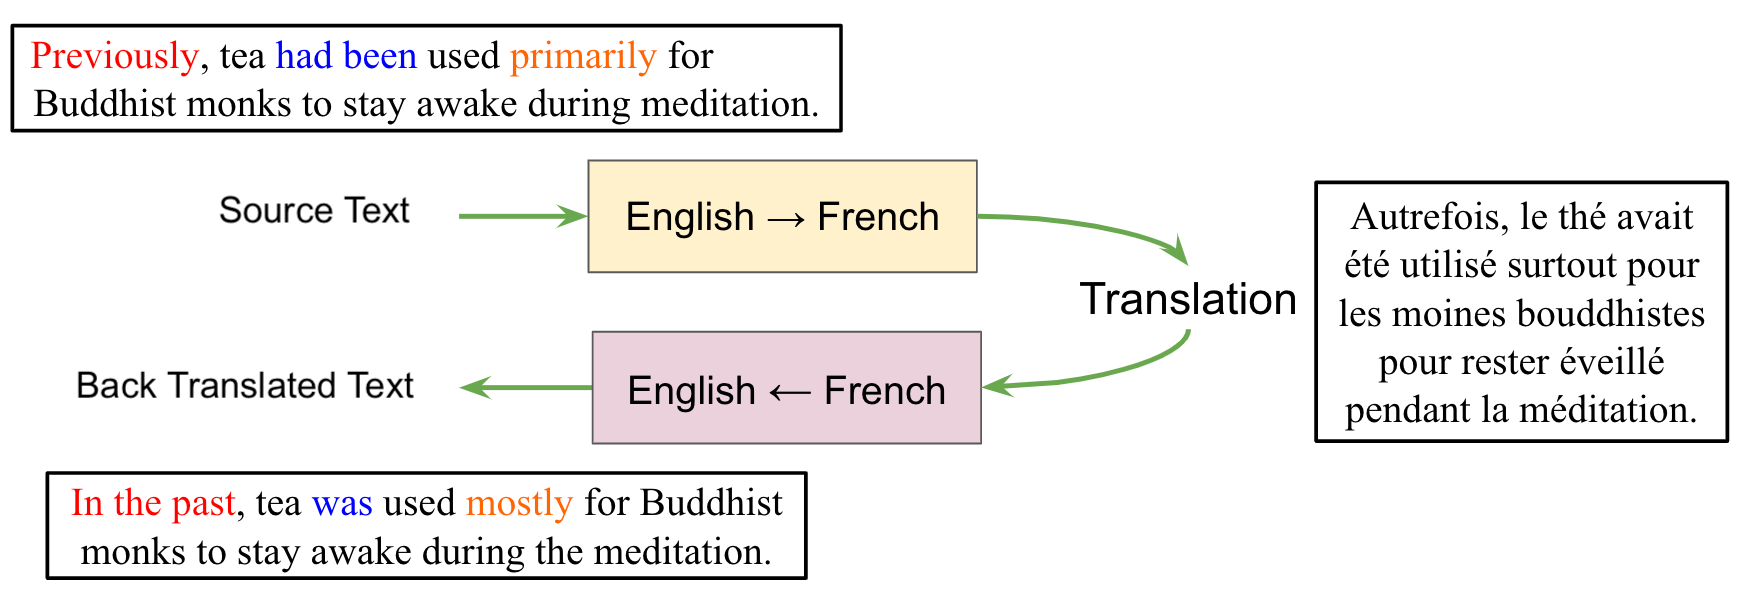
\includegraphics[height=5cm,width=1.0\linewidth]{figures/back-translation.png}
  \caption{Example of Back Translation (best viewed in color)}
\label{figureBT}
\end{figure}

Back translation is recommended in the domains where the content subjected to translation is too sensitive and needs to be double-checked. The back-translation method is widely used in medical research and clinical trials, as it is required by Ethics Committees and regulatory authorities in several countries~\cite{whyBT}. This allows us to compare the back-translated text with the original text to evaluate the quality of the translation.  

The rationale behind using back-translation is that for sensitive documents in the medical domain, back-translation is a recommended practice to cross-verify that the translation adheres to the intended meaning. Usually, back-translation is mandatory in case of quality assessment of medical consent forms, so this is not an overhead in this particular scenario and is generally recommended for medical, legal, market research, and government agencies working in public health, safety, and legal matters. We are utilizing this for translation evaluation. We aim to address the specific needs of these domains to ensure the faithfulness of the translated texts. Our efforts are to use already available back-translation texts for the translation evaluation tasks. 




% \subsection{Knowledge Graphs}
% Knowledge graphs represent structured collections of facts describing the world in the form of relationships between entities~\cite{knowledgegrphs}.  KGs are a popular model for representing static, graph-structured data. Formally, a KG is a graph-based representation model, where nodes represent entities and edges represent relations between these entities~\cite{knowledgegrphs}, 
% shaped as a set of triples: ``for a given set of entities $\mathcal{E}$ and set of relations $\mathcal{R}$, we consider a knowledge graph $\mathcal{K} \subseteq K = \mathcal{E} \times \mathcal{R} \times \mathcal{E}$ as a directed, multi-relational graph that comprises triples $(h, r, t) \in \mathcal{K}$ in which $h, t \in \mathcal{E}$ represent a triple's respective head and tail entities and $r \in \mathcal{R}$ represents its relationship''\cite{KG2}.

\subsection{Resource Description Framework}\label{rdfintro}

The Resource Description Framework (RDF) is a W3C standard for data representation on the Web. RDF provides a foundation for encoding information in a structured way for the Semantic Web~\cite{RDF}. It is particularly useful for representing knowledge about entities and the relationships between them.


\subsubsection{Components of RDF}

RDF consists of triplets, which are fundamental units of information. These triplets, also known as RDF triples, form the building blocks for representing knowledge within an RDF graph. Each RDF triple is composed of three elements:

\begin{enumerate}
  \item \textbf{Subject:} The resource (entity) being described. (e.g., ``The patient'')
  \item \textbf{Predicate:} The property or characteristic of the subject, denoted by directed arrows. (e.g., ``has diagnosisof'')
  \item \textbf{Object:} The value associated with the predicate for the subject. (e.g., ``pneumonia'')
\end{enumerate}

\begin{figure}[h]
  \centering
  
\includegraphics[height=0.7cm,width=0.45\linewidth]{figures/rdftriple.jpg}
  \caption{RDF Triple for the sentence ``The patient has diagnosis of pneumonia''}
  \label{rdffigure}
\end{figure}

In Figure~\ref{rdffigure}, the RDF triple depicts a statement about a patient having a diagnosis of pneumonia. In the context of our research, we leverage RDF to capture the semantics of the sentences, enabling a more nuanced evaluation of translation quality compared to traditional metrics.

\subsubsection{FRED RDF Graphs}

Our research is based on RDF graphs provided by FRED (Framework for RDF-based Extraction and Disambiguation)~\cite{fredPaper} to capture semantic nuances in translated texts. At its core, FRED leverages the Resource Description Framework (RDF) to construct semantic graphs that capture the relationships and entities present in the text. FRED bridges the gap between unstructured text and structured knowledge representation, employing Semantic Web technologies to extract and disambiguate information from textual data. Figure~\ref{fdadrug} shows the RDF graph for the sentence ``An experimental drug is one which has not been approved by FDA.''.

% \textbf{!Explain why fred simplified graphs are required and not the actual rdf graphs}

\begin{figure}[h]
  \centering
  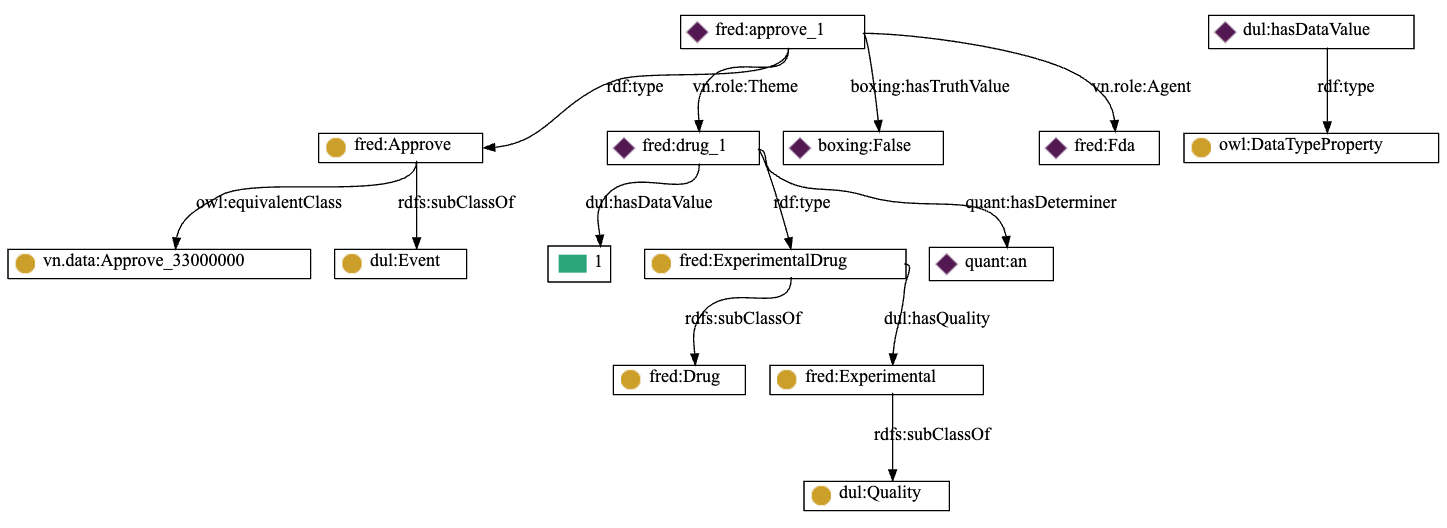
\includegraphics[height=5cm, width=1\linewidth]{figures/rdf-fda.png}
  \caption{FRED RDF graph for “An experimental drug is one which has not been approved by FDA.” taken from a medical consent form.}
  \label{fdadrug}
\end{figure}

% Rather than comparing RDF XML graphs (which adds lots of complexities in the graphs), we should just compare the simplified graph (like the ones below). (EXPLAIN RDF XML)

% \begin{figure}[h]
%   \centering
%   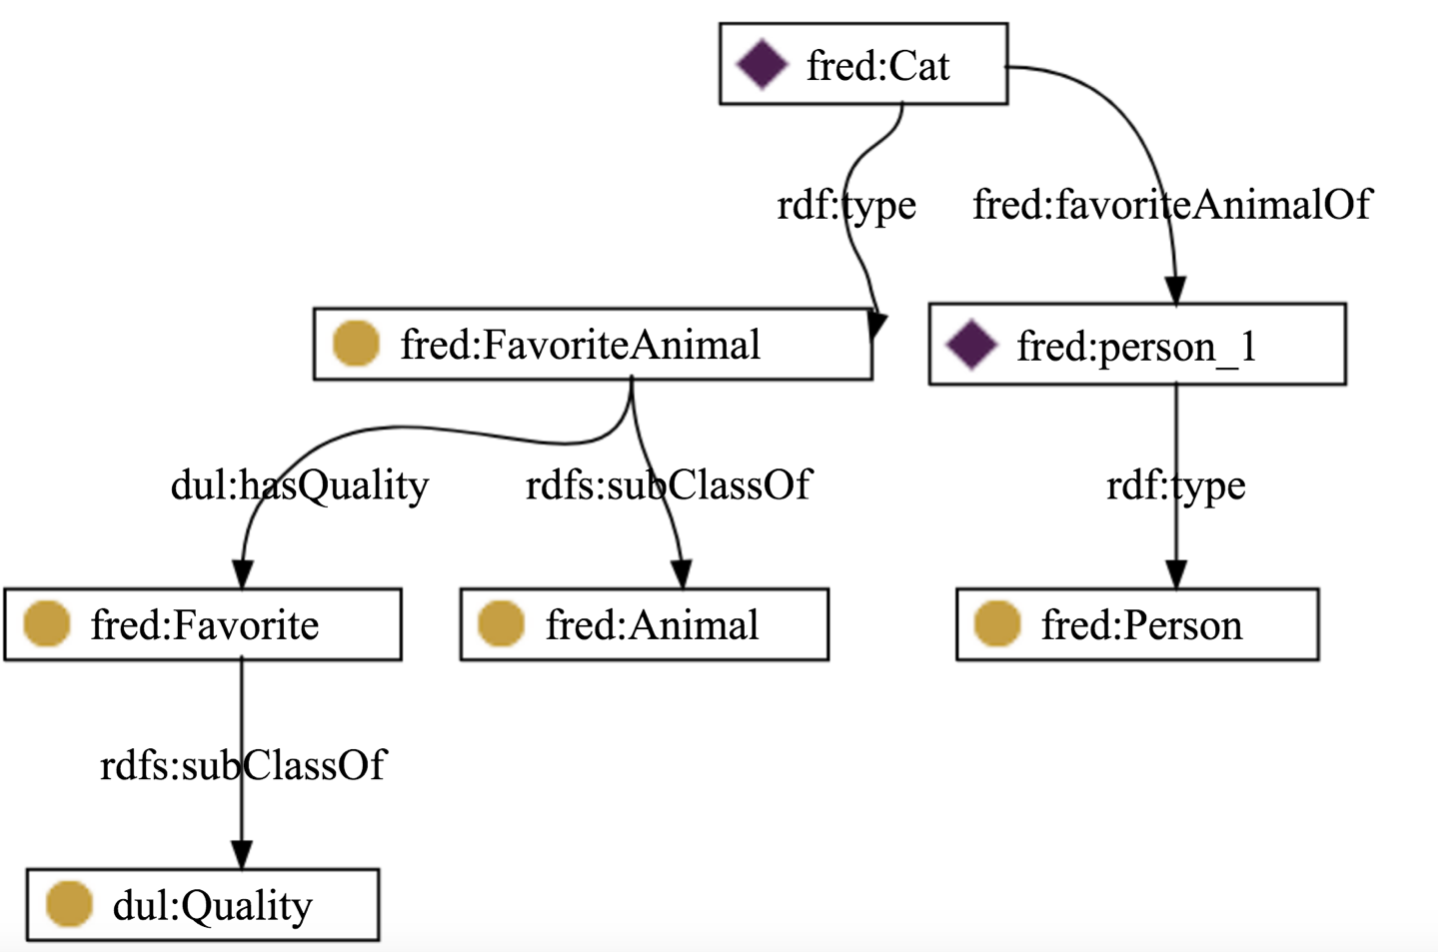
\includegraphics[height=10cm,width=1\linewidth]{figures/rdf_cat_favorite.png}
%   \caption{RDF Simplified Schema for sentence: ‘Cat is my favorite animal’ using RDF Text Example (Using FRED (wit.istc.cnr.it/stlab-tools/fred/demo/))}
%   \label{cat}
%   \end{figure}


% VINAY
% Methodologies
% 1. Proposed method (RDF metric, novel work)
% 2. Motivation behind using RDF
% 3. Design of the experiments, Data sets,
% preprocessing (Creating RDF graph, cleaning it, and comparing)
% 4. How the metric is working (mechanism)


\section{Experiment Design}\label{experiments}

We conduct a comparative experiment to evaluate the efficacy of our proposed RDF-based evaluation metric, GATE, in comparison to the baseline metric BLEU and its correlation with human judgment. To obtain baseline BLEU scores, we are using iBLEU~\cite{ibleu}. The evaluation procedure, outlined in Algorithm~\ref{algo}, explains the comparison of RDF graphs generated through the FRED API, which can be accessed at http://wit.istc.cnr.it/stlab-tools/fred/demo/.


\subsection{Dataset}

Our experiments were done on the selected medical consent forms and the sentences from Semantic Textual Similarity (STS) Benchmark Dataset~\cite{STSdata} to evaluate the effectiveness of GATE in capturing semantic similarity compared to BLEU.~The medical consent forms dataset has around 250 original sentence, their corresponding translations, and the back-translated texts, all provided by human translators. Due to the selected availability of medical data, we augmented our analysis with the STS benchmark dataset. In total, our experiments were conducted on 500 sentence pairs, with 250 pairs sourced from medical consent forms provided by a medical institute.

% , which provides source text, translated text, and reference text for translation evaluation task. 

%---------------------------------------------------

% \subsection{Graph Edit Distance in RDF Graphs}

% \begin{figure}[h]
% \centering
% \includegraphics[height=10cm,width=0.8\linewidth]{figures/rdf_graph_cat.png}
% \caption{RDF XML Graph for 'There is a cat on the mat'. This figure is just to showcase the complexity of RDF graphs for simple sentences.}
% \end{figure}
% We are using NX library for Graph Edit Distance. 
% There are various algorithms for comparing the GED.
% As we can see in Fig 4.3, RDF graphs tends to be very complicated even for simple sentences.


% Due to this there is a very poor correlation between the semantic comparison of the sentences as seen below.

% Here is the graph [Fig 4.4] for score comparison.

% \begin{figure}[h]
% \centering
% \includegraphics[height=10cm,width=1\linewidth]{figures/result.png}
% \caption{Sentence pair ids and their corresponding BLEU, RDF\_similarity, Ground Truth scores}
% \end{figure}

%-----------------------------------------


% \subsection{Pre-processing}
% Source text, getting the back-translation
% Talking about the data sets here
% Using FRED API to get the RDF graph in XML format. Figure \#n shows the simplified RDF graph for a sentence from a medical consent form for a drug trial. We are using FRED (REF??) (FRED is a tool for automatically producing RDF/OWL ontologies and linked data from natural language sentences). The method is based on Discourse Representation Theory, Ontology Design Patterns etc. Results are enriched with Named Entity Resolution (NER) and Word-Sense Disambiguation (WSD).

\subsection{Graph comparison and GATE Score}

We are comparing the source sentence with the back-translated text by constructing RDF graphs for both. The distance between graphs is measured as the Jaccard similarity coefficient~\cite{jaccard} between the entities in the graphs. This way, the distance between the source and the back-translated sentence graph is normalized between 0 and 1, where 1 denotes an exact match, and 0 denotes no similarity. Algorithm~\ref{algo} outlines the steps in the evaluation process. Specifically, for source sentence $\mathbf{s}_k$, and the back-translated text $\mathbf{b}_k$, the GATE Score is calculated as follows:

\[{G}_{k} = \cfrac{entities(\mathbf{s}_k)\cap entities(\mathbf{b}_k)}{entities(\mathbf{s}_k)\cup entities(\mathbf{b}_k)}\]



% For Graph comparison we are using Jaccard similarity as defined below:

% \textbf{Jaccard Similarity}: Jaccard similarity is a measure of similarity between two sets. It is defined as the size of the intersection of the sets divided by the size of the union of the sets. In the context of translation quality estimation, Jaccard similarity can be used to quantify the similarity between the two RDF Graphs based on the presence or absence of RDF nodes.

% We are calculating the evaluation score via Jaccard similarity defined as:

% We are applying Jaccard similarity to RDF graphs to compare the source and back-translated text. 
% Evaluation score is jaccard similarity score.

% The Jaccard similarity coefficient, denoted by $J(A, B)$, between sets $A$ and $B$ is calculated as:

% \[
% J(A, B) = \frac{|A \cap B|}{|A \cup B|}
% \]

% where $|A \cap B|$ represents the cardinality of the intersection of sets $A$ and $B$, and $|A \cup B|$ represents the cardinality of the union of sets $A$ and $B$.


\begin{algorithm}
  \caption{: GATE Score evaluation process}
  \begin{algorithmic}[1]
  \Require All source sentences $\mathbf{s}_k \in \mathbf{S}$ and target sentences $\mathbf{t}_k \in \mathbf{T}$ of $n$ sentence pairs
  \Ensure sentence-level scores $\mathbf{G}_k$
  \For{each sentence pair $\{\mathbf{s}_k, \mathbf{t}_k\} \in \{\mathbf{S}, \mathbf{T}\}$}
      \State $\mathbf{b}_k \gets$ back-translation of $\mathbf{t}_k$ (either already available or obtained using Google Translate)
      \\
      \State $entities(\mathbf{s}_k) \gets$ RDF graph nodes of
      %  (entities) the source sentence 
      $\mathbf{s}_k$ 
      using FRED 
      % API
      
      \State $entities(\mathbf{b}_k) \gets$ RDF graph nodes of 
      % (entities) the back-translated sentence 
      $\mathbf{b}_k$ 
      using FRED 
      %  API
\\

\State $\mathbf{common} \gets \{x\,\mid\, x \in entities(\mathbf{s}_k)$  \textbf{and}  $x \in entities(\mathbf{b}_k)\}$

\State $\mathbf{unison} \gets \{x\,\mid\, x \in entities(\mathbf{s}_k)$  \textbf{or}  $x \in entities(\mathbf{b}_k)\}$

\\
\State $\mathbf{G}_{k} \gets \cfrac{common}{unison}$ 
  \\
  \EndFor
  \end{algorithmic}
  \label{algo}
\end{algorithm}



\begin{figure}[h]
  \centering
  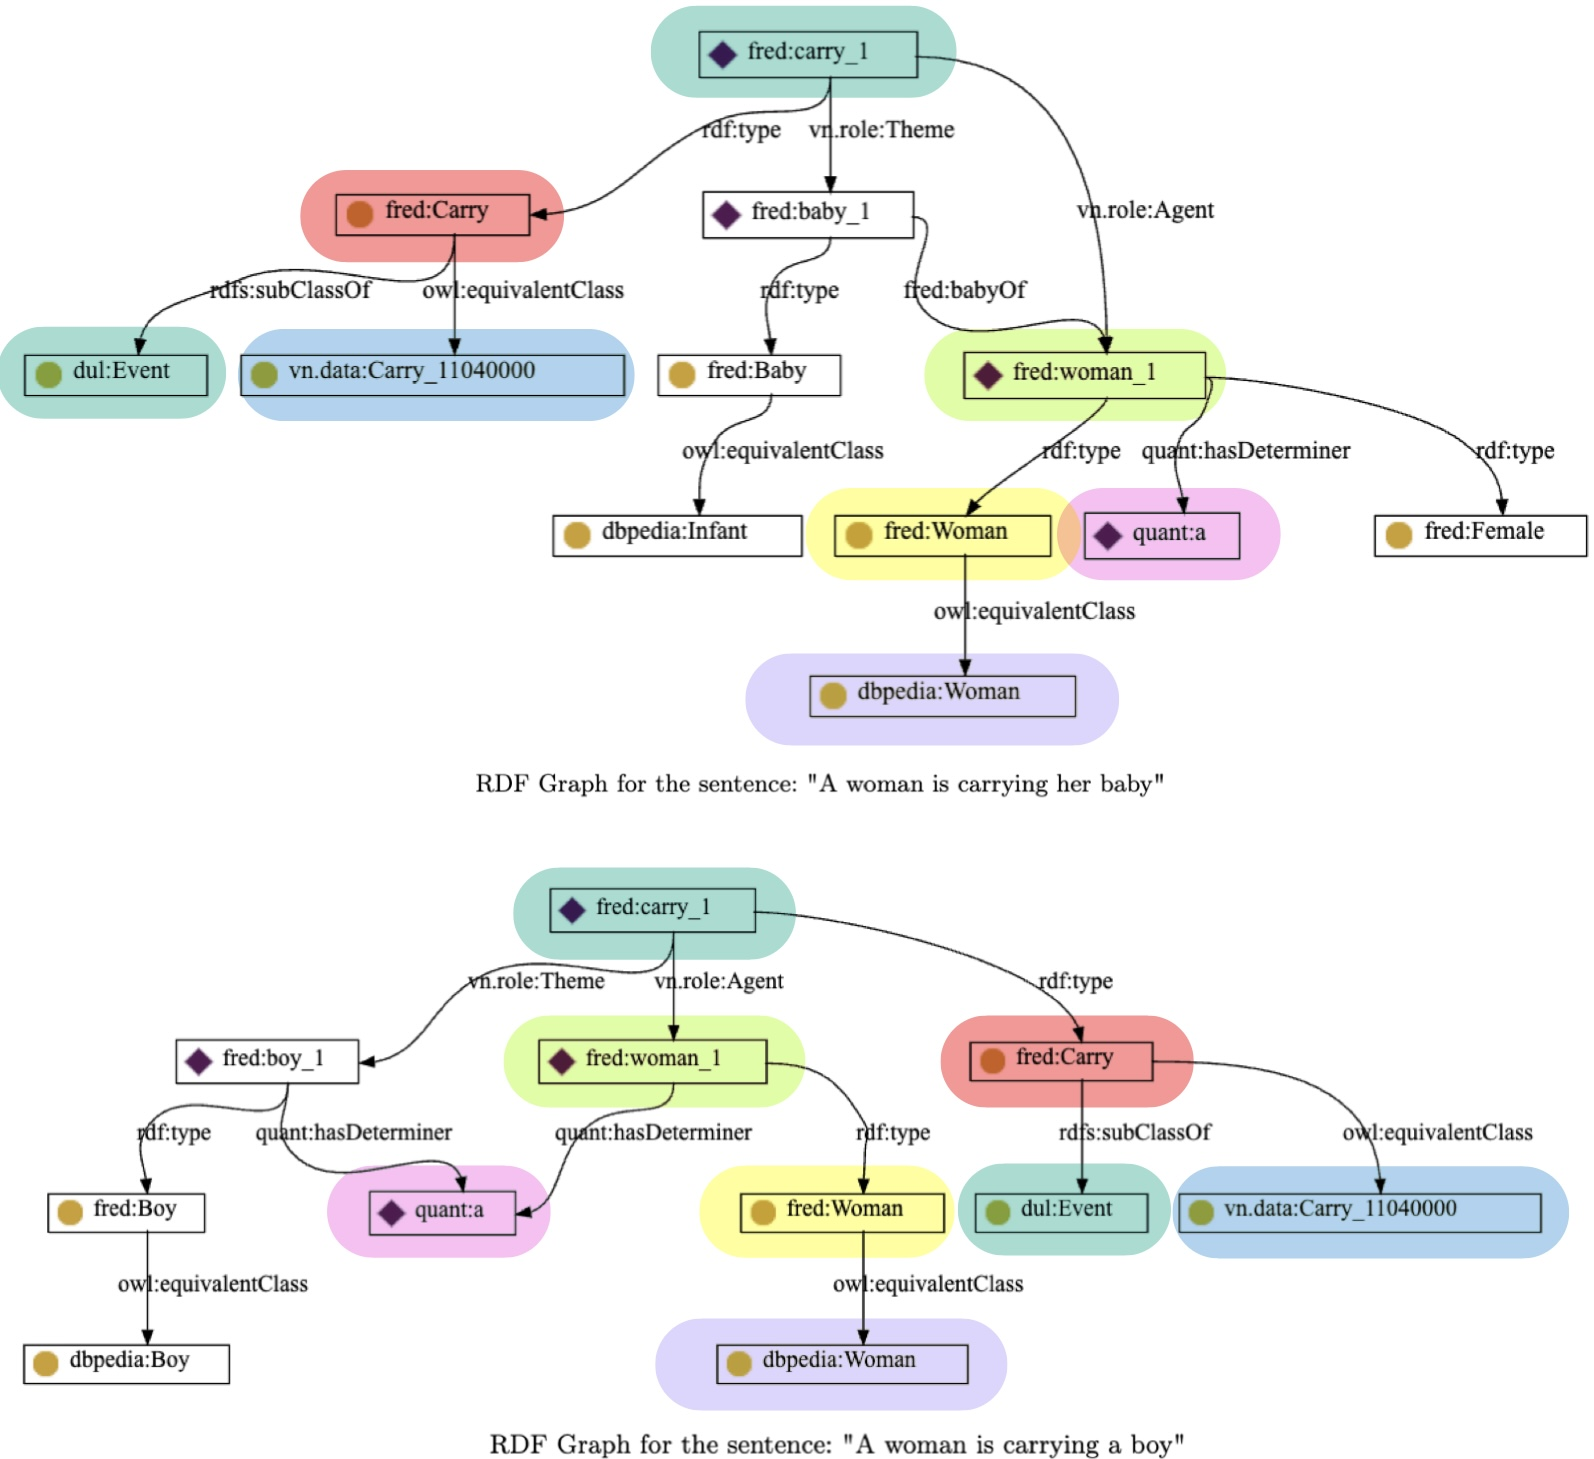
\includegraphics[height=10cm,width=1\linewidth]{figures/graphcompare2.jpg}
  \caption{Graph Comparison for measuring semantic similarity. Common nodes are highlighted in multiple colors. In these two graphs there are 8 common nodes, and total unique nodes are 15.~(best viewed in color)}
  \label{graphcompare}
  \end{figure}



% \subsection{GATE Score}



% \pagebreak



% \textbf{two exmples of long sentences from the dataset with bleu and gate score}

In the next section, we present the findings of our experiments along with a discussion of the insights gained from our research efforts while also addressing the current limitations of our metric.

% \pagebreak


\section{Results \& Discussion}\label{results}

Our experiment implemented the proposed GATE metric alongside the baseline metric, BLEU.~We calculated the Pearson correlation between the BLEU score and GATE score against human judgment on the experiment dataset. Our results in Table~\ref{score}, show that GATE achieves a significantly higher correlation with human judgment in translation evaluation tasks compared to the widely used metric, BLEU.~Specifically, GATE exhibits a approximately 70\% improvement in correlation on the experiment data, with a Pearson correlation coefficient of 0.357 compared to BLEU's 0.200. The higher correlation underscores the effectiveness of leveraging RDF graphs in capturing semantic information, thereby improvement in correlation with human judgments. 

\begin{table}[h]
  \centering
  \caption{System-wide Pearson correlation of BLEU and GATE with human judgments on MCFs Data and STS Benchmark Dataset}
  \begin{tabular}{|l|c|c}
    \hline 
  Metric & Pearson Correlation \\
  \hline
  
  BLEU   & 0.200                            \\
  \hline 
  GATE   & \textbf{0.357}    \\
  \hline                        
  \end{tabular}
  \label{score}
\end{table}

% \begin{table}
%   \caption{GATE vs. BLEU score against human evaluation. Selected examples from the experiment run on STS dataset.
%   %  in the interval [0,1] with 1 denoting the best possible correlation.
%   Higher correlation with human judgment are marked in bold.
%     % \textcolor{orange}{ !Should 'Gold Score' be renamed as 'Human judgment'?}
%     }
%   \begin{tabular}{cllccccc}
%     \toprule
%     Serial&Hypothesis&Reference&Human&GATE&BLEU\\
%     \midrule
%     1.&A man is erasing a chalk board & The man is erasing the chalk board & \textit{\textcolor{teal}{1.00}} & \textbf{0.65} & 0.60 \\
%     2.&Three men are playing guitars & Three men on stage are playing guitars & \textit{\textcolor{teal}{0.75}} & 0.45 & \textbf{0.60} \\
%     3.&A woman is carrying a boy & A woman is carrying her baby & \textit{\textcolor{teal}{0.47}} & \textbf{0.53} & 0.63 \\
%     4.&A woman peels a potato & A woman is peeling a potato. & \textit{\textcolor{teal}{1.00}} & \textbf{1.00} & 0.52 \\
%     \bottomrule
%   \end{tabular}
%   \label{examples}
% \end{table}

Table~\ref{examples} shows examples with corresponding human evaluation scores, GATE scores, and BLEU scores. These examples serve to highlight GATE's capability to better reflect human perception of semantic similarity, as evidenced by its closer alignment with human judgments compared to BLEU scores. In summary, our findings indicate that integrating RDF graphs with already existing back-translated texts holds promise for reference-free translation evaluation. This metric can potentially assist human evaluators who evaluate the translation of sensitive documents using back-translated texts.

\pagebreak

For the Figure~\ref{graphcompare}, the GATE Score is calculated as: 

\[{G} = \cfrac{8 \text{ (number of common entities)}}{15 \text{ (total unique nodes in both the graphs)}} = 0.53\]

\begin{table}
  \caption{GATE vs. BLEU score against human evaluation. \\Selected examples from the experiment run on STS dataset.
  %  in the interval [0,1] with 1 denoting the best possible correlation.
  Higher correlation with human judgment is marked in bold.
    % \textcolor{orange}{ !Should 'Gold Score' be renamed as 'Human judgment'?}
    }
    \begin{tabular}{llccccc}
  \hline    % \toprule
      Hypothesis&Reference&Human&GATE&BLEU\\
      \hline %\midrule
      A man is erasing a chalk board & The man is erasing the chalk board & \textit{1.00} & \textbf{0.65} & 0.60 \\
      Three men are playing guitars & Three men on stage are playing guitars & \textit{0.75} & 0.45 & \textbf{0.60} \\
      A woman is carrying a boy & A woman is carrying her baby & \textit{0.47} & \textbf{0.53} & 0.63 \\
      A woman peels a potato & A woman is peeling a potato. & \textit{1.00} & \textbf{1.00} & 0.52 \\
      \hline %\bottomrule
    \end{tabular}
    \label{examples}
  \end{table}


Using RDF for translation evaluation could be helpful as they `encode' real-world semantics akin to how embeddings work in neural network frameworks (such as COMET), contrasting with metrics that are based on lexical level information for translation evaluation (such as BLEU). This work has the potential to pave the way for utilizing knowledge graphs in the field of translation evaluation alongside existing resources, such as word embeddings and LLM-based frameworks. Our experiments reinforce our belief, demonstrating that using knowledge graphs to encode meaning is helpful and gets better results than the baseline metrics.

Given that RDF is currently available only in English and our metric compares graphs of original and back-translated texts for translation evaluation, our metric is presently only applicable where English is the source language. However, the target language can be any other language as long as back-translation is available.

While our results do not surpass state-of-the-art performance, they serve as a proof-of-concept, showcasing the effectiveness of leveraging RDF graphs for translation evaluation tasks. As FRED accommodates large sentences as well, our future work will involve working with more extensive real-world translated medical data and testing our methodology on larger sentences to demonstrate its effectiveness comprehensively. These results underscore the advantages of GATE over traditional metrics like BLEU and motivate further validation of GATE's applicability on real-world data particularly in domains like medicine, along with continuing our exploration for further improvement of the metric. 

% \subsection{Translation Evaluation for English to any language}
% Reproducibility: 
% We will release the code-base and detailed step by step process described in this paper to the research community upon publication, along with the detailed scripts to get the required RDF graphs. 


% \section{Discussion}
% Using Knowledge Graphs for Translation Evaluation could be useful as they ‘encode’ real world semantics just like how the embeddings work in neural network frameworks unlike metrics which rely upon lexical level information for translation quality assessment. Our metric  can be used where English is the source language and target language could be any language where back-translation is available. We are introducing a novel approach for translation evaluation in the context of back-translation which is usually available for medical and legal domain. It may assist the human evaluators who are checking the sensitive documents using back translation. 


% We believe that this work will pave the way for utilizing knowledge graphs in the field of translation evaluation, alongside other existing resources such as word embeddings, LLM-Based frameworks. Our belief is reinforced by our initial experiments which shows that using knowledge graphs for encoding the meaning could be useful and get better results than the baseline metrics like BLEU. 

% Our proposed approach strength is that it correlates better with human judgment than BLEU. 

% Finally since Translation and Summarization can both be viewed as natural language generation from a textual context, we believe Knowledge Graphs could be adapted to evaluating summarization or similar natural language generation tasks. 

% \textbf{TODO articulating the limitations and combining Limitations with discussions}
% % \subsection{Limitations}
% % Does not beat state of the art like COMET etc. 


\section{Conclusion}\label{conclusion}

% VINAY
% % Conclusion & Future work
% 1. Summary of key points
% 2. RDF is working well in some context, novel approach
% 3. Future work: how RDF can be strengthened (other languages apart from English)
% 4. Creating a software to automate integrating the translation and back-translation texts and rdf graph creation and rdf comparison

In this paper, we introduce GATE, a novel metric based on the Resource Description Framework (RDF) designed for assessing the quality of translated medical texts for which back-translation is available. To showcase the effectiveness of our metric, we conducted experiments using selected medical data and the STS benchmark dataset, comparing the results against the baseline metric, BLEU, and human judgment scores. Notably, GATE exhibits a stronger correlation with human judgment than BLEU, achieving a higher Pearson correlation coefficient (0.357 compared to BLEU's 0.200), representing approximately a \textasciitilde70\% improvement over BLEU, the most commonly used metric. 

By leveraging back-translation and using RDF graphs to encode both semantic and syntactical information, GATE provides a reference-less and semantically aware assessment of translation quality. In comparison with the more advanced Large Language Model (LLM)-based metrics such as COMET, our metric is computationally much lighter. It works for any target language, including low-resource languages, and does not require any data training. Our research shows that, in the field of translation evaluation, existing resources like back-translation and Resource Description Framework could be helpful in real-world scenarios such as the medical domain.

% Our research shows that existing resource like Back Translation and Knowledge Graphs (such as RDF) have the potential to improve the translation evaluation metrics.

% TODO
% Our metric surpasses BLEU specifically in the context of sensitive medical and legal documents, where semantic accuracy is paramount.

% ======


\section{Future Directions}\label{future}


As part of future work, we would like to explore:

\begin{enumerate}
  \item Conducting further experiments to validate the efficacy of GATE on real-world translated medical data.
  \item Since Translation and Summarization can both be viewed as natural language generation from a textual context, we aim to explore knowledge graphs such as RDF in the area of evaluating summarization or similar natural language generation tasks. Investigate the utilization of knowledge graphs for tasks beyond translation evaluation, such as summarization.
  \item For calculating GATE score, experimenting with different formulas incorporating variations in weights of entities, incoming edges, and outgoing edges.
  \item Addressing the challenge of language dependency in GATE by incorporating multilingual knowledge graphs since FRED works only with English texts. A primary avenue for future work, will be looking into the inclusion of other knowledge graphs available in other languages, making GATE language independent.
 \item Development of a software similar to iBLEU for integrating FRED API to facilitate automatic scoring of source and back-translated texts, enhanced visualization, and accessibility of the RDF metric.
  \item~\cite{btfuture} shows that back-translation could be useful for improving the translation quality for low-resource languages. Our future work is to combine neural networks with back-translation and knowledge graphs in the area of translation evaluation for low-resource languages. Our future work aims to combine these technologies along with knowledge graphs (such as Knowledge Graph Embeddings) to improve our metric, making it suitable for evaluating translated sensitive texts and investigating the potential of combining neural networks with back-translation and knowledge graphs to improve translation quality, particularly for low-resource languages.
\end{enumerate}

% \section{First Section}
% % \subsection{A Subsection Sample}
% % Please note that the first paragraph of a section or subsection is
% % not indented. The first paragraph that follows a table, figure,
% % equation etc. does not need an indent, either.

% % Subsequent paragraphs, however, are indented.

% \subsubsection{Sample Heading (Third Level)} Only two levels of
% headings should be numbered. Lower level headings remain unnumbered;
% they are formatted as run-in headings.

% \paragraph{Sample Heading (Fourth Level)}
% The contribution should contain no more than four levels of
% headings. Table~\ref{tab1} gives a summary of all heading levels.

% \begin{table}
% \caption{Table captions should be placed above the
% tables.}\label{tab1}
% \begin{tabular}{|l|l|l|}
% \hline
% Heading level &  Example & Font size and style\\
% \hline
% Title (centered) &  {\Large\bfseries Lecture Notes} & 14 point, bold\\
% 1st-level heading &  {\large\bfseries 1 Introduction} & 12 point, bold\\
% 2nd-level heading & {\bfseries 2.1 Printing Area} & 10 point, bold\\
% 3rd-level heading & {\bfseries Run-in Heading in Bold.} Text follows & 10 point, bold\\
% 4th-level heading & {\itshape Lowest Level Heading.} Text follows & 10 point, italic\\
% \hline
% \end{tabular}
% \end{table}


% \noindent Displayed equations are centered and set on a separate
% line.
% \begin{equation}
% x + y = z
% \end{equation}
% Please try to avoid rasterized images for line-art diagrams and
% schemas. Whenever possible, use vector graphics instead (see
% Fig.~\ref{fig1}).

% \begin{figure}
% 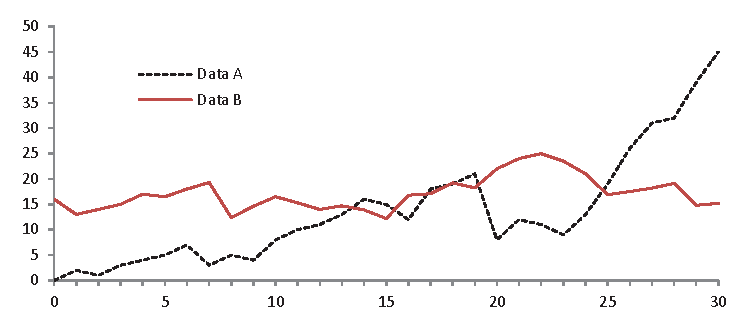
\includegraphics[width=\textwidth]{fig1.eps}
% \caption{A figure caption is always placed below the illustration.
% Please note that short captions are centered, while long ones are
% justified by the macro package automatically.} \label{fig1}
% \end{figure}

% \begin{theorem}
% This is a sample theorem. The run-in heading is set in bold, while
% the following text appears in italics. Definitions, lemmas,
% propositions, and corollaries are styled the same way.
% \end{theorem}
% %
% % the environments 'definition', 'lemma', 'proposition', 'corollary',
% % 'remark', and 'example' are defined in the LLNCS documentclass as well.
% %
% \begin{proof}
% Proofs, examples, and remarks have the initial word in italics,
% while the following text appears in normal font.
% \end{proof}
% For citations of references, we prefer the use of square brackets
% and consecutive numbers. Citations using labels or the author/year
% convention are also acceptable. The following bibliography provides
% a sample reference list with entries for journal
% articles~\cite{ref_article1}, an LNCS chapter~\cite{ref_lncs1}, a
% book~\cite{ref_book1}, proceedings without editors~\cite{ref_proc1},
% and a homepage~\cite{ref_url1}. Multiple citations are grouped
% \cite{ref_article1,ref_lncs1,ref_book1},
% \cite{ref_article1,ref_book1,ref_proc1,ref_url1}.

\paragraph*{Supplemental Material Statement:} 
Source code for Algorithm~\ref{algo} is available from Github\footnote{https://github.com/vinayneekhra/GATE}. 
Selected Medical Consent Forms Dataset cannot be made available as it incorporates private data. However, STS Benchmark Dataset used in the experiment is publicly available.

\begin{credits}
\subsubsection{\ackname}Our sincere gratitude to the late Prof. Ravi Kothari, on whose suggestions this research work was started. We thank anonymous reviewers for their time and valuable suggestions for improving the paper. We also express our gratitude to  Supriya Ranjan, Bhavesh Neekhra, Mamatha Alugubelly, and others for their invaluable feedback and support.  

% \subsubsection{\discintname}
% It is now necessary to declare any competing interests or to specifically
% state that the authors have no competing interests. Please place the
% statement with a bold run-in heading in small font size beneath the
% (optional) acknowledgments\footnote{If , our proceedings submission
% system, is used, then the disclaimer can be provided directly in the system.},
% for example: The authors have no competing interests to declare that are
% relevant to the content of this article. Or: Author A has received research
% grants from Company W. Author B has received a speaker honorarium from
% Company X and owns stock in Company Y. Author C is a member of committee Z.
\end{credits}
%
% ---- Bibliography ----
%
% BibTeX users should specify bibliography style 'splncs04'.
% References will then be sorted and formatted in the correct style.
%
\bibliographystyle{splncs04}
\bibliography{mybibliography}
%
% \begin{thebibliography}{8}

% \begin{splncs04}{8}



% \end{thebibliography}
\end{document}

% \bibitem{ref_article1}
% Author, F.: Article title. Journal \textbf{2}(5), 99--110 (2016)

% \bibitem{ref_lncs1}
% Author, F., Author, S.: Title of a proceedings paper. In: Editor,
% F., Editor, S. (eds.) CONFERENCE 2016, LNCS, vol. 9999, pp. 1--13.
% Springer, Heidelberg (2016). \doi{10.10007/1234567890}

% \bibitem{ref_book1}
% Author, F., Author, S., Author, T.: Book title. 2nd edn. Publisher,
% Location (1999)

% \bibitem{ref_proc1}
% Author, A.-B.: Contribution title. In: 9th International Proceedings
% on Proceedings, pp. 1--2. Publisher, Location (2010)

% \bibitem{ref_url1}
% LNCS Homepage, \url{http://www.springer.com/lncs}, last accessed 2023/10/25

